\chapter{Introdução}\label{chp:introducao}
O objetivo deste texto é propor algumas atividades práticas para a consolidação dos conceitos abordados na disciplina Redes de Comunicação I. Essa disciplina é oferecida na Faculdade de Tecnologia da Universidade Estadual de Campinas (FT/UNICAMP) para os cursos Bacharelado em Sistemas de Informação e Tecnologia em Análise e Desenvolvimento de Sistemas.

Esse material pode ser utilizado por qualquer pessoa, de qualquer curso ou instituição, desde que respeitadas as condições da licença CC-BY-4.0, descrita na \Cpageref{chp:licenca}. Informações de como obter o material também estão nessa página.

Supõe-se que o estudante leitor deste material já tenha instalado o \CPT. Caso ainda não tenha instalado, o estudante poderá fazê-lo a partir dos passos a seguir:

\begin{enumerate}[label*=\arabic*.]
    \item Acesse o site \url{https://www.netacad.com/courses/packet-tracer}
    \item Agora, você deve cadastrar-se no site.
    \begin{enumerate}[label*=\arabic*.]
        \item No canto superior direito, clique na opção \enquote{\textit{login}}.
        \item Na parte inferior da nova página, Registre-se.
    \end{enumerate}
    \item Depois de cadastrado e já na sua área, clique na opção \enquote{Recursos} e, em seguida, \enquote{Baixar o Packet Tracer}.
    \item No final da nova página carregada, escolha a versão mais adequada para o sistema operacional que você vai utilizar.
\end{enumerate}

Se a instalação aconteceu corretamente, execute o \CPT. A tela inicial do software deve ser parecida com aquela ilustrada na \Cref{fig:telaInicial}. Note que há duas visões possíveis para a rede que vamos montar ou simular: a visão lógica (\textit{Logical}) e a visão física (\textit{Physical}). Nós vamos nos concentrar na visão lógica.

\begin{figure}[!htb]
    \centering
    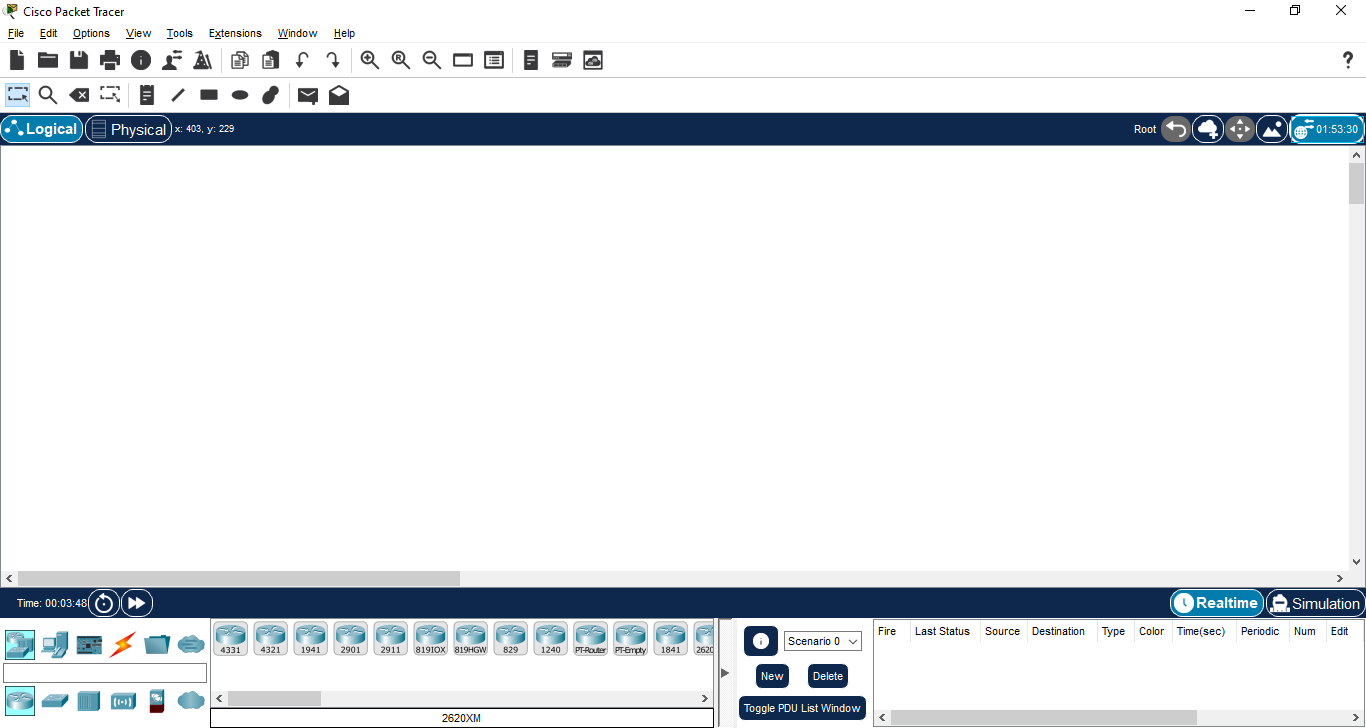
\includegraphics[width=.99\textwidth]{Figuras/TelaInicial}
    \caption{Tela inicial do \CPT.}    \label{fig:telaInicial}
\end{figure}

Ainda na tela da \Cref{fig:telaInicial}, na parte de baixo, à esquerda, note que temos vários elementos para as redes de comunicação. Esses elementos vão desde dispositivos internos da rede (\textit{Network Devices}) até dispositivos finais (\textit{End Devices}), incluindo os elementos para as conexões (cabeamento). Utilizaremos esses elementos nos exercícios ao longo deste tutorial.

\section{Exercício}
Como exercício, familiarize-se com os elementos que compõem uma rede de computadores. Usando o \CPT, tente identificar os seguintes elementos:
\begin{itemize}
    \item Roteadores, \textit{switches} e \textit{hubs}.
    \item PCs, \textit{notebooks} e servidores.
    \item Dispositivos para internet das coisas (por exemplo, um detector de monóxido de carbono \textit{online}).
    \item Cabo coaxial, cabo de cobre (par trançado), cabo de cobre \textit{cross-over}, fibra óptica.
\end{itemize}